\documentclass[border=6pt]{standalone}
\usepackage{fontspec,unicode-math}
\setmainfont{Noto Sans}
\setsansfont{Noto Sans}
\setmathfont{STIXTwoMath-Regular.otf}
\usepackage{tikz}
\usetikzlibrary{arrows.meta,calc,intersections,patterns,decorations.markings}
\definecolor{ScienceInk}{HTML}{000000}
\definecolor{ScienceCurve}{HTML}{000000}
\definecolor{ScienceAlt}{HTML}{A36035}
\tikzset{axis/.style={draw=ScienceInk,line width=.68pt,>=Latex},
 trace/.style={draw=ScienceCurve,line width=1.42pt,line cap=round,line join=round},
 secondary/.style={draw=ScienceAlt,line width=1.25pt,dashed,line cap=round},
 energy/.style={draw=ScienceInk,line width=1.35pt,line cap=round},
 shiftline/.style={draw=ScienceAlt,densely dashed,line width=1.1pt},
 photon/.style={->,draw=ScienceCurve,line width=1.10pt,>=Latex},
 lab/.style={text=ScienceInk,font=\fontsize{13}{16}\selectfont,inner sep=1.5pt},
 smalllab/.style={text=ScienceInk,font=\fontsize{11}{14}\selectfont,inner sep=1pt},
 panellab/.style={font=\fontsize{13}{16}\itshape,text=ScienceInk,inner sep=0pt}}
\begin{document}


% Figure 6.6: schematic spectral diffusion; no experimental units were provided.
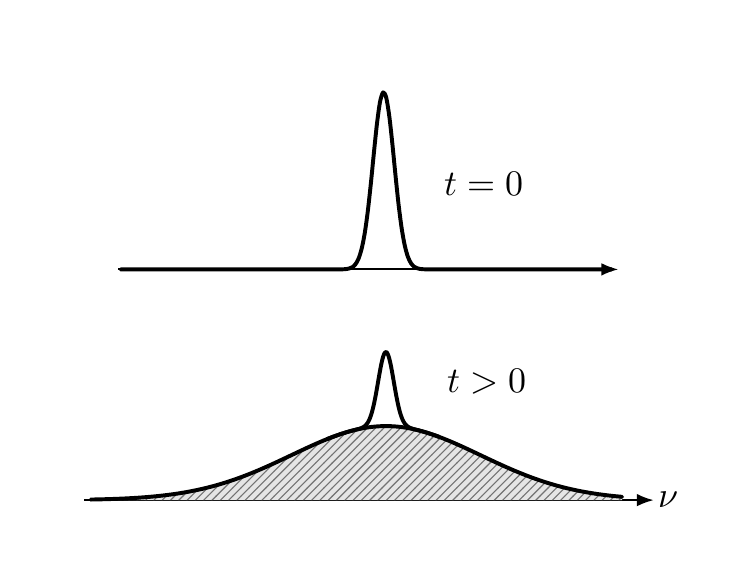
\begin{tikzpicture}[x=1cm,y=1cm]
  \path[use as bounding box] (0,0) rectangle (8.6,6.55);
  % first snapshot (t=0)
  \draw[axis,->] (1.15,3.48)--(7.50,3.48);
  \draw[trace,smooth,domain=1.18:7.42,samples=160,variable=\x]
    plot (\x,{3.48+2.25*exp(-((\x-4.52)/.19)^2)});
  \node[lab,anchor=west] at (5.24,4.56) {$t=0$};
  % second snapshot (t>0), broad redistributed packet is shaded, narrow residual remains
  \draw[axis,->] (0.72,.55)--(7.95,.55);
  \fill[ScienceCurve!10] plot[domain=.8:7.55,samples=100,variable=\x]
    (\x,{.55+.94*exp(-((\x-4.55)/1.70)^2)}) --(7.55,.55)--(.8,.55)--cycle;
  \begin{scope}
    \clip (.77,.55) rectangle (7.60,1.63);
    \fill[pattern=north east lines,pattern color=ScienceInk!55] plot[domain=.8:7.55,samples=90,variable=\x]
      (\x,{.55+.94*exp(-((\x-4.55)/1.70)^2)}) --(7.55,.55)--(.8,.55)--cycle;
  \end{scope}
  \draw[trace,smooth,domain=.8:7.55,samples=160,variable=\x]
    plot (\x,{.55+.94*exp(-((\x-4.55)/1.70)^2)});
  \draw[trace,smooth,domain=3.80:5.22,samples=150,variable=\x]
    plot (\x,{.55+.94*exp(-((\x-4.55)/1.70)^2)+.94*exp(-((\x-4.55)/.14)^2)});
  \node[lab,anchor=west] at (5.27,2.06) {$t>0$};
  \node[lab,anchor=west] at (7.95,.56) {$\nu$};
\end{tikzpicture}

\end{document}
